\documentclass[a4paper]{book}
\usepackage{makeidx}
\usepackage{natbib}
\usepackage{graphicx}
\usepackage{multicol}
\usepackage{float}
\usepackage{listings}
\usepackage{color}
\usepackage{ifthen}
\usepackage[table]{xcolor}
\usepackage{textcomp}
\usepackage{alltt}
\usepackage{ifpdf}
\ifpdf
\usepackage[pdftex,
            pagebackref=true,
            colorlinks=true,
            linkcolor=blue,
            unicode
           ]{hyperref}
\else
\usepackage[ps2pdf,
            pagebackref=true,
            colorlinks=true,
            linkcolor=blue,
            unicode
           ]{hyperref}
\usepackage{pspicture}
\fi
\usepackage[utf8]{inputenc}
\usepackage{polski}
\usepackage[T1]{fontenc}

\usepackage{mathptmx}
\usepackage[scaled=.90]{helvet}
\usepackage{courier}
\usepackage{sectsty}
\usepackage[titles]{tocloft}
\usepackage{doxygen}
\lstset{language=C++,inputencoding=utf8,basicstyle=\footnotesize,breaklines=true,breakatwhitespace=true,tabsize=8,numbers=left }
\makeindex
\setcounter{tocdepth}{3}
\renewcommand{\footrulewidth}{0.4pt}
\renewcommand{\familydefault}{\sfdefault}
\hfuzz=15pt
\setlength{\emergencystretch}{15pt}
\hbadness=750
\tolerance=750
\begin{document}
\hypersetup{pageanchor=false,citecolor=blue}
\begin{titlepage}
\vspace*{7cm}
\begin{center}
{\Large \-Graf }\\
\vspace*{1cm}
{\large \-Wygenerowano przez Doxygen 1.7.6.1}\\
\vspace*{0.5cm}
{\small Sun May 11 2014 23:21:11}\\
\end{center}
\end{titlepage}
\clearemptydoublepage
\pagenumbering{roman}
\tableofcontents
\clearemptydoublepage
\pagenumbering{arabic}
\hypersetup{pageanchor=true,citecolor=blue}
\chapter{\-Struktura katalogów}
\section{\-Katalogi}
\-Ta struktura katalogów jest posortowana jest z grubsza, choć nie całkowicie, alfabetycznie\-:\begin{DoxyCompactList}
\item \contentsline{section}{prj}{\pageref{dir_9f92f53661fd78c561fa1672d6c740cd}}{}
\end{DoxyCompactList}

\chapter{\-Indeks klas}
\section{\-Lista klas}
\-Tutaj znajdują się klasy, struktury, unie i interfejsy wraz z ich krótkimi opisami\-:\begin{DoxyCompactList}
\item\contentsline{section}{\hyperlink{class_drzewo}{\-Drzewo$<$ K, W $>$} \\*\-Modeluje pojecie drzewa binarnego. \-Jego atrybutem jest klasa \hyperlink{class_wezel}{\-Wezel} }{\pageref{class_drzewo}}{}
\item\contentsline{section}{\hyperlink{class_para}{\-Para$<$ K, W $>$} \\*\-Modeluje pojecie pary. \-Jej atrybutem sa pola zawierajace klucz i wartosci }{\pageref{class_para}}{}
\item\contentsline{section}{\hyperlink{class_tablica}{\-Tablica$<$ K, W $>$} \\*\-Modeluje pojecie tablicy z haszowaniem. \-Klasa modeluje pojecie tablicy z haszowaniem. \-Jej atrybutami sa pola\-: klucz i wartosc }{\pageref{class_tablica}}{}
\item\contentsline{section}{\hyperlink{class_wezel}{\-Wezel$<$ K, W $>$} \\*\-Modeluje pojecie wezla. \-Jego atrybutem jest klasa \hyperlink{class_para}{\-Para} }{\pageref{class_wezel}}{}
\end{DoxyCompactList}

\chapter{\-Indeks plików}
\section{\-Lista plików}
\-Tutaj znajduje się lista wszystkich plików z ich krótkimi opisami\-:\begin{DoxyCompactList}
\item\contentsline{section}{\hyperlink{main_8cpp}{main.\-cpp} \\*\-Plik zawiera glowna funkcje programu }{\pageref{main_8cpp}}{}
\item\contentsline{section}{\hyperlink{simplex_8cpp}{simplex.\-cpp} \\*\-Definicje poszczegolnych funkcji dla klasy \hyperlink{class_simplex}{\-Simplex} }{\pageref{simplex_8cpp}}{}
\item\contentsline{section}{\hyperlink{simplex_8h}{simplex.\-h} \\*\-Plik naglowkowy klasy \hyperlink{class_simplex}{\-Simplex} }{\pageref{simplex_8h}}{}
\end{DoxyCompactList}

\chapter{\-Dokumentacja katalogów}
\hypertarget{dir_3823f649f201ab38ac9f9627a6a7b058}{\section{\-Dokumentacja katalogu /home/martyna/pamsi2/graf/prj/inc/}
\label{dir_3823f649f201ab38ac9f9627a6a7b058}\index{\-Dokumentacja katalogu /home/martyna/pamsi2/graf/prj/inc/@{\-Dokumentacja katalogu /home/martyna/pamsi2/graf/prj/inc/}}
}
\-Directory dependency graph for /home/martyna/pamsi2/graf/prj/inc/\-:\nopagebreak
\begin{figure}[H]
\begin{center}
\leavevmode
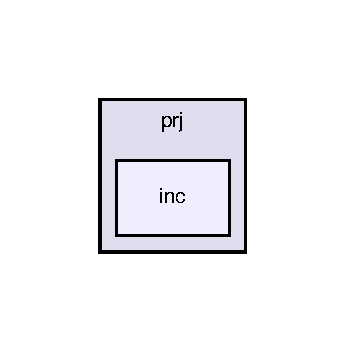
\includegraphics[width=166pt]{dir_3823f649f201ab38ac9f9627a6a7b058_dep}
\end{center}
\end{figure}
\subsection*{\-Pliki}
\begin{DoxyCompactItemize}
\item 
plik \hyperlink{benchmark_8h}{benchmark.\-h}
\begin{DoxyCompactList}\small\item\em \-Plik naglowkowy \-Benchmark. \end{DoxyCompactList}\item 
plik \hyperlink{graf_8h}{graf.\-h}
\begin{DoxyCompactList}\small\item\em \-Plik naglowkowy klasy \-Graf.\-Klasa \hyperlink{class_graf}{\-Graf} zawierajaca definicje poszczegolnych funkcji. \end{DoxyCompactList}\item 
plik \hyperlink{szukajki_8h}{szukajki.\-h}
\begin{DoxyCompactList}\small\item\em \-Plik zawiera definicje funkcji szukajki. \end{DoxyCompactList}\end{DoxyCompactItemize}

\hypertarget{dir_01d7db6dcbd9ee9eb2513e350ed3be5b}{\section{\-Dokumentacja katalogu /home/martyna/pamsi2/graf/prj/}
\label{dir_01d7db6dcbd9ee9eb2513e350ed3be5b}\index{\-Dokumentacja katalogu /home/martyna/pamsi2/graf/prj/@{\-Dokumentacja katalogu /home/martyna/pamsi2/graf/prj/}}
}
\-Directory dependency graph for /home/martyna/pamsi2/graf/prj/\-:\nopagebreak
\begin{figure}[H]
\begin{center}
\leavevmode
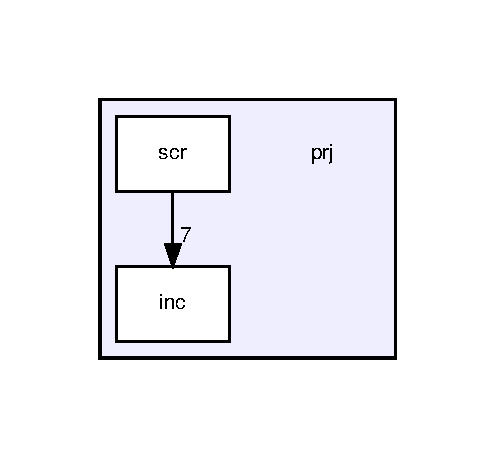
\includegraphics[width=238pt]{dir_01d7db6dcbd9ee9eb2513e350ed3be5b_dep}
\end{center}
\end{figure}
\subsection*{\-Katalogi}
\begin{DoxyCompactItemize}
\item 
katalog \hyperlink{dir_3823f649f201ab38ac9f9627a6a7b058}{inc}
\item 
katalog \hyperlink{dir_02f7d643b664388aa50f6742704a651d}{scr}
\end{DoxyCompactItemize}

\hypertarget{dir_02f7d643b664388aa50f6742704a651d}{\section{\-Dokumentacja katalogu /home/martyna/pamsi2/graf/prj/scr/}
\label{dir_02f7d643b664388aa50f6742704a651d}\index{\-Dokumentacja katalogu /home/martyna/pamsi2/graf/prj/scr/@{\-Dokumentacja katalogu /home/martyna/pamsi2/graf/prj/scr/}}
}
\-Directory dependency graph for /home/martyna/pamsi2/graf/prj/scr/\-:\nopagebreak
\begin{figure}[H]
\begin{center}
\leavevmode
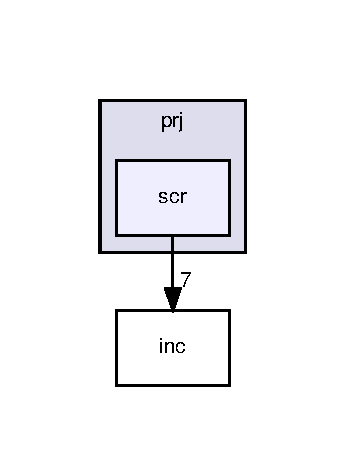
\includegraphics[width=166pt]{dir_02f7d643b664388aa50f6742704a651d_dep}
\end{center}
\end{figure}
\subsection*{\-Pliki}
\begin{DoxyCompactItemize}
\item 
plik \hyperlink{benchmark_8cpp}{benchmark.\-cpp}
\begin{DoxyCompactList}\small\item\em \-Benchmark \-Zawiera fukcje programu liczaca czas przeszukiwan poszczegolnych pomiarow. \end{DoxyCompactList}\item 
plik \hyperlink{graf_8cpp}{graf.\-cpp}
\begin{DoxyCompactList}\small\item\em \-Definicje poszczegolnych funkcji dla klasy \hyperlink{class_graf}{\-Graf}. \end{DoxyCompactList}\item 
plik \hyperlink{main_8cpp}{main.\-cpp}
\begin{DoxyCompactList}\small\item\em \-Plik zawiera glowna funkcje programu. \end{DoxyCompactList}\item 
plik \hyperlink{szukajki_8cpp}{szukajki.\-cpp}
\begin{DoxyCompactList}\small\item\em \-Szukajki \-Zawiera najważniejsze fukcje programu. \-Trzy przeszukiwania grafu -\/ depth first, breadth first, \-A$\ast$. \end{DoxyCompactList}\end{DoxyCompactItemize}

\chapter{\-Dokumentacja klas}
\hypertarget{class_graf}{\section{\-Dokumentacja klasy \-Graf}
\label{class_graf}\index{\-Graf@{\-Graf}}
}


\-Deklaracja klasy \hyperlink{class_graf}{\-Graf}.  




{\ttfamily \#include $<$graf.\-h$>$}

\subsection*{\-Metody publiczne}
\begin{DoxyCompactItemize}
\item 
\hyperlink{class_graf_a697a2852c7f65779f23e30fd0e8dd081}{\-Graf} (int \hyperlink{class_graf_aac4d211e752539963f002d255991f5b4}{rozm})
\item 
\hyperlink{class_graf_a4ff3904fd04f367ac0219b52719c567e}{$\sim$\-Graf} ()
\item 
bool \hyperlink{class_graf_a27d67c3b74894008a177b4a6b3a5a8ec}{dod\-\_\-wierz} (int v)
\item 
bool \hyperlink{class_graf_a9f9097c607ea725e4aaf738fb6c4fa49}{dod\-\_\-kraw} (int v1, int v2, double c)
\item 
bool \hyperlink{class_graf_aa2a49b2df35ed0f4c308696bf21694f6}{usun\-\_\-kraw} (int v1, int v2)
\item 
bool \hyperlink{class_graf_a670df5348dbd4cf3bcc8c223cb04e10f}{usun\-\_\-wierz} (int v)
\item 
double \hyperlink{class_graf_adc0aaf7f7f62343b149538c63c61deda}{czy\-\_\-sasiad} (int v1, int v2)
\item 
std\-::list$<$ int $>$ \hyperlink{class_graf_a98e19234c0961a4e42dda003cbabd274}{sasiedztwo} (int v)
\item 
const int \hyperlink{class_graf_ab452377f7bf7a7034057c9b1c1f2c4fb}{rozmiar} () const 
\end{DoxyCompactItemize}
\subsection*{\-Atrybuty prywatne}
\begin{DoxyCompactItemize}
\item 
double \hyperlink{class_graf_aa9bee9eccd66c284e079ba25d7519dcb}{dane} \mbox{[}1000\mbox{]}\mbox{[}1000\mbox{]}
\item 
int \hyperlink{class_graf_aac4d211e752539963f002d255991f5b4}{rozm}
\end{DoxyCompactItemize}


\subsection{\-Opis szczegółowy}


\-Definicja w linii 13 pliku graf.\-h.



\subsection{\-Dokumentacja konstruktora i destruktora}
\hypertarget{class_graf_a697a2852c7f65779f23e30fd0e8dd081}{\index{\-Graf@{\-Graf}!\-Graf@{\-Graf}}
\index{\-Graf@{\-Graf}!Graf@{\-Graf}}
\subsubsection[{\-Graf}]{\setlength{\rightskip}{0pt plus 5cm}{\bf \-Graf\-::\-Graf} (
\begin{DoxyParamCaption}
\item[{int}]{rozm}
\end{DoxyParamCaption}
)}}\label{class_graf_a697a2852c7f65779f23e30fd0e8dd081}


\-Definicja w linii 22 pliku graf.\-cpp.

\hypertarget{class_graf_a4ff3904fd04f367ac0219b52719c567e}{\index{\-Graf@{\-Graf}!$\sim$\-Graf@{$\sim$\-Graf}}
\index{$\sim$\-Graf@{$\sim$\-Graf}!Graf@{\-Graf}}
\subsubsection[{$\sim$\-Graf}]{\setlength{\rightskip}{0pt plus 5cm}{\bf \-Graf\-::$\sim$\-Graf} (
\begin{DoxyParamCaption}
{}
\end{DoxyParamCaption}
)}}\label{class_graf_a4ff3904fd04f367ac0219b52719c567e}


\-Definicja w linii 24 pliku graf.\-cpp.



\subsection{\-Dokumentacja funkcji składowych}
\hypertarget{class_graf_adc0aaf7f7f62343b149538c63c61deda}{\index{\-Graf@{\-Graf}!czy\-\_\-sasiad@{czy\-\_\-sasiad}}
\index{czy\-\_\-sasiad@{czy\-\_\-sasiad}!Graf@{\-Graf}}
\subsubsection[{czy\-\_\-sasiad}]{\setlength{\rightskip}{0pt plus 5cm}double {\bf \-Graf\-::czy\-\_\-sasiad} (
\begin{DoxyParamCaption}
\item[{int}]{v1, }
\item[{int}]{v2}
\end{DoxyParamCaption}
)}}\label{class_graf_adc0aaf7f7f62343b149538c63c61deda}


\-Definicja w linii 41 pliku graf.\-cpp.



\-Oto graf wywoływań tej funkcji\-:\nopagebreak
\begin{figure}[H]
\begin{center}
\leavevmode
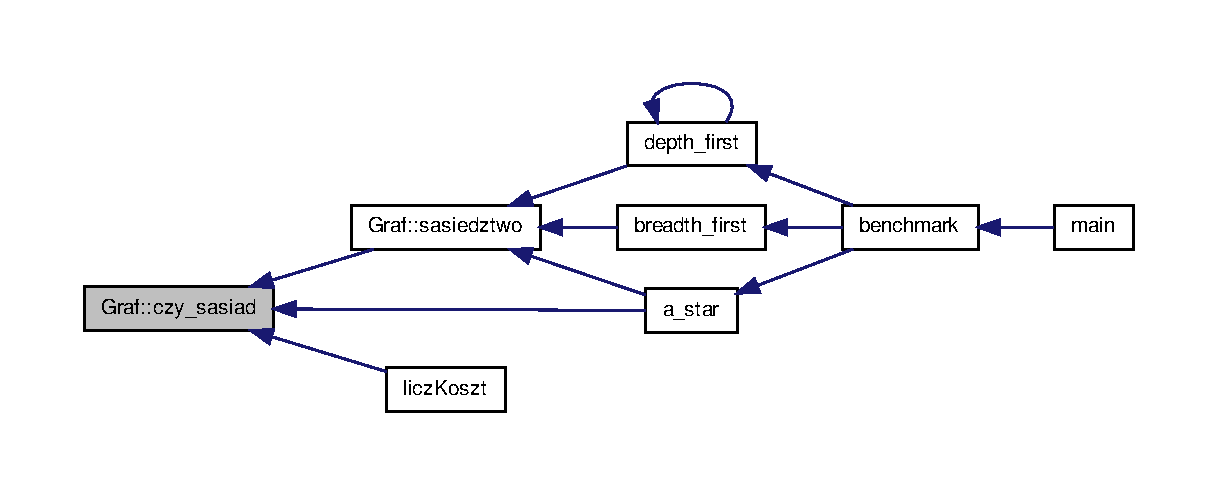
\includegraphics[width=350pt]{class_graf_adc0aaf7f7f62343b149538c63c61deda_icgraph}
\end{center}
\end{figure}


\hypertarget{class_graf_a9f9097c607ea725e4aaf738fb6c4fa49}{\index{\-Graf@{\-Graf}!dod\-\_\-kraw@{dod\-\_\-kraw}}
\index{dod\-\_\-kraw@{dod\-\_\-kraw}!Graf@{\-Graf}}
\subsubsection[{dod\-\_\-kraw}]{\setlength{\rightskip}{0pt plus 5cm}bool {\bf \-Graf\-::dod\-\_\-kraw} (
\begin{DoxyParamCaption}
\item[{int}]{v1, }
\item[{int}]{v2, }
\item[{double}]{c}
\end{DoxyParamCaption}
)}}\label{class_graf_a9f9097c607ea725e4aaf738fb6c4fa49}


\-Definicja w linii 28 pliku graf.\-cpp.



\-Oto graf wywoływań tej funkcji\-:\nopagebreak
\begin{figure}[H]
\begin{center}
\leavevmode
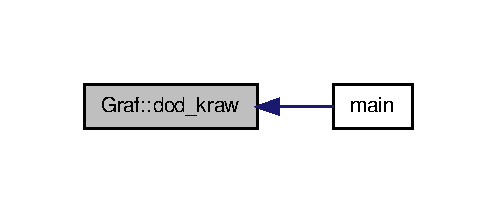
\includegraphics[width=238pt]{class_graf_a9f9097c607ea725e4aaf738fb6c4fa49_icgraph}
\end{center}
\end{figure}


\hypertarget{class_graf_a27d67c3b74894008a177b4a6b3a5a8ec}{\index{\-Graf@{\-Graf}!dod\-\_\-wierz@{dod\-\_\-wierz}}
\index{dod\-\_\-wierz@{dod\-\_\-wierz}!Graf@{\-Graf}}
\subsubsection[{dod\-\_\-wierz}]{\setlength{\rightskip}{0pt plus 5cm}bool {\bf \-Graf\-::dod\-\_\-wierz} (
\begin{DoxyParamCaption}
\item[{int}]{v}
\end{DoxyParamCaption}
)}}\label{class_graf_a27d67c3b74894008a177b4a6b3a5a8ec}


\-Definicja w linii 25 pliku graf.\-cpp.

\hypertarget{class_graf_ab452377f7bf7a7034057c9b1c1f2c4fb}{\index{\-Graf@{\-Graf}!rozmiar@{rozmiar}}
\index{rozmiar@{rozmiar}!Graf@{\-Graf}}
\subsubsection[{rozmiar}]{\setlength{\rightskip}{0pt plus 5cm}const int {\bf \-Graf\-::rozmiar} (
\begin{DoxyParamCaption}
{}
\end{DoxyParamCaption}
) const}}\label{class_graf_ab452377f7bf7a7034057c9b1c1f2c4fb}


\-Definicja w linii 51 pliku graf.\-cpp.



\-Oto graf wywoływań tej funkcji\-:\nopagebreak
\begin{figure}[H]
\begin{center}
\leavevmode
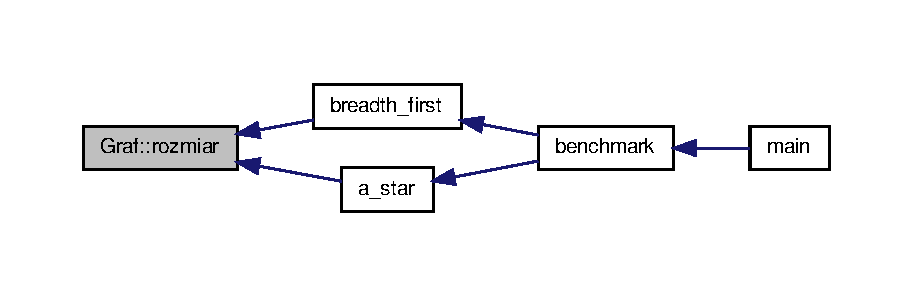
\includegraphics[width=350pt]{class_graf_ab452377f7bf7a7034057c9b1c1f2c4fb_icgraph}
\end{center}
\end{figure}


\hypertarget{class_graf_a98e19234c0961a4e42dda003cbabd274}{\index{\-Graf@{\-Graf}!sasiedztwo@{sasiedztwo}}
\index{sasiedztwo@{sasiedztwo}!Graf@{\-Graf}}
\subsubsection[{sasiedztwo}]{\setlength{\rightskip}{0pt plus 5cm}std\-::list$<$ int $>$ {\bf \-Graf\-::sasiedztwo} (
\begin{DoxyParamCaption}
\item[{int}]{v}
\end{DoxyParamCaption}
)}}\label{class_graf_a98e19234c0961a4e42dda003cbabd274}


\-Definicja w linii 44 pliku graf.\-cpp.



\-Oto graf wywołań dla tej funkcji\-:\nopagebreak
\begin{figure}[H]
\begin{center}
\leavevmode
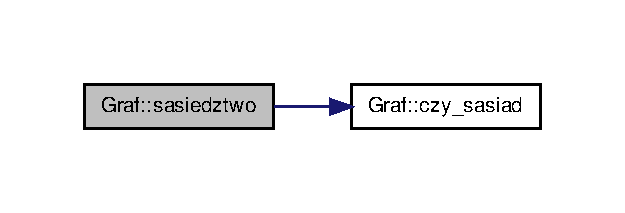
\includegraphics[width=300pt]{class_graf_a98e19234c0961a4e42dda003cbabd274_cgraph}
\end{center}
\end{figure}




\-Oto graf wywoływań tej funkcji\-:\nopagebreak
\begin{figure}[H]
\begin{center}
\leavevmode
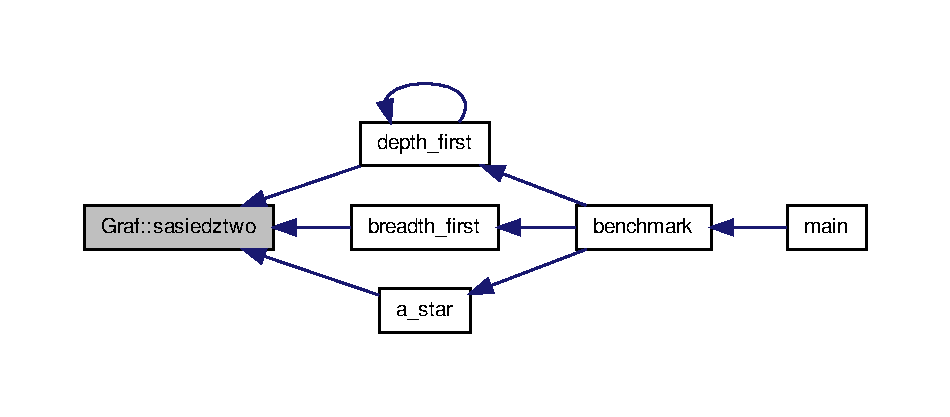
\includegraphics[width=350pt]{class_graf_a98e19234c0961a4e42dda003cbabd274_icgraph}
\end{center}
\end{figure}


\hypertarget{class_graf_aa2a49b2df35ed0f4c308696bf21694f6}{\index{\-Graf@{\-Graf}!usun\-\_\-kraw@{usun\-\_\-kraw}}
\index{usun\-\_\-kraw@{usun\-\_\-kraw}!Graf@{\-Graf}}
\subsubsection[{usun\-\_\-kraw}]{\setlength{\rightskip}{0pt plus 5cm}bool {\bf \-Graf\-::usun\-\_\-kraw} (
\begin{DoxyParamCaption}
\item[{int}]{v1, }
\item[{int}]{v2}
\end{DoxyParamCaption}
)}}\label{class_graf_aa2a49b2df35ed0f4c308696bf21694f6}


\-Definicja w linii 33 pliku graf.\-cpp.

\hypertarget{class_graf_a670df5348dbd4cf3bcc8c223cb04e10f}{\index{\-Graf@{\-Graf}!usun\-\_\-wierz@{usun\-\_\-wierz}}
\index{usun\-\_\-wierz@{usun\-\_\-wierz}!Graf@{\-Graf}}
\subsubsection[{usun\-\_\-wierz}]{\setlength{\rightskip}{0pt plus 5cm}bool {\bf \-Graf\-::usun\-\_\-wierz} (
\begin{DoxyParamCaption}
\item[{int}]{v}
\end{DoxyParamCaption}
)}}\label{class_graf_a670df5348dbd4cf3bcc8c223cb04e10f}


\-Definicja w linii 38 pliku graf.\-cpp.



\subsection{\-Dokumentacja atrybutów składowych}
\hypertarget{class_graf_aa9bee9eccd66c284e079ba25d7519dcb}{\index{\-Graf@{\-Graf}!dane@{dane}}
\index{dane@{dane}!Graf@{\-Graf}}
\subsubsection[{dane}]{\setlength{\rightskip}{0pt plus 5cm}double {\bf \-Graf\-::dane}\mbox{[}1000\mbox{]}\mbox{[}1000\mbox{]}\hspace{0.3cm}{\ttfamily  \mbox{[}private\mbox{]}}}}\label{class_graf_aa9bee9eccd66c284e079ba25d7519dcb}


\-Definicja w linii 14 pliku graf.\-h.

\hypertarget{class_graf_aac4d211e752539963f002d255991f5b4}{\index{\-Graf@{\-Graf}!rozm@{rozm}}
\index{rozm@{rozm}!Graf@{\-Graf}}
\subsubsection[{rozm}]{\setlength{\rightskip}{0pt plus 5cm}int {\bf \-Graf\-::rozm}\hspace{0.3cm}{\ttfamily  \mbox{[}private\mbox{]}}}}\label{class_graf_aac4d211e752539963f002d255991f5b4}


\-Definicja w linii 15 pliku graf.\-h.



\-Dokumentacja dla tej klasy została wygenerowana z plików\-:\begin{DoxyCompactItemize}
\item 
\hyperlink{graf_8h}{graf.\-h}\item 
\hyperlink{graf_8cpp}{graf.\-cpp}\end{DoxyCompactItemize}

\chapter{\-Dokumentacja plików}
\hypertarget{benchmark_8cpp}{\section{\-Dokumentacja pliku benchmark.\-cpp}
\label{benchmark_8cpp}\index{benchmark.\-cpp@{benchmark.\-cpp}}
}


\-Benchmark \-Zawiera fukcje programu liczaca czas przeszukiwan poszczegolnych pomiarow.  


{\ttfamily \#include \char`\"{}graf.\-h\char`\"{}}\*
{\ttfamily \#include \char`\"{}szukajki.\-h\char`\"{}}\*
{\ttfamily \#include $<$iostream$>$}\*
{\ttfamily \#include $<$chrono$>$}\*
\-Wykres zależności załączania dla benchmark.\-cpp\-:\nopagebreak
\begin{figure}[H]
\begin{center}
\leavevmode
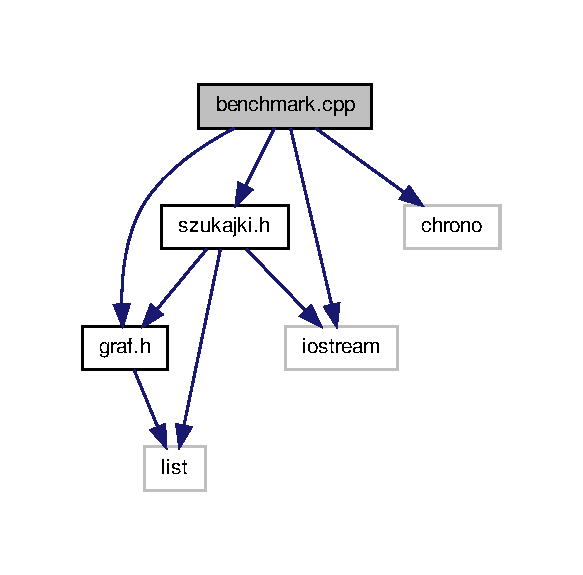
\includegraphics[width=280pt]{benchmark_8cpp__incl}
\end{center}
\end{figure}
\subsection*{\-Funkcje}
\begin{DoxyCompactItemize}
\item 
void \hyperlink{benchmark_8cpp_a4a33bba40119da5e2debd21d9ab45cdb}{benchmark} (\hyperlink{class_graf}{\-Graf} \&cos, int poczatek, int koniec, std\-::ostream \&out)
\end{DoxyCompactItemize}


\subsection{\-Opis szczegółowy}


\-Definicja w pliku \hyperlink{benchmark_8cpp_source}{benchmark.\-cpp}.



\subsection{\-Dokumentacja funkcji}
\hypertarget{benchmark_8cpp_a4a33bba40119da5e2debd21d9ab45cdb}{\index{benchmark.\-cpp@{benchmark.\-cpp}!benchmark@{benchmark}}
\index{benchmark@{benchmark}!benchmark.cpp@{benchmark.\-cpp}}
\subsubsection[{benchmark}]{\setlength{\rightskip}{0pt plus 5cm}void {\bf benchmark} (
\begin{DoxyParamCaption}
\item[{{\bf \-Graf} \&}]{cos, }
\item[{int}]{poczatek, }
\item[{int}]{koniec, }
\item[{std\-::ostream \&}]{out}
\end{DoxyParamCaption}
)}}\label{benchmark_8cpp_a4a33bba40119da5e2debd21d9ab45cdb}


\-Definicja w linii 15 pliku benchmark.\-cpp.



\-Oto graf wywołań dla tej funkcji\-:\nopagebreak
\begin{figure}[H]
\begin{center}
\leavevmode
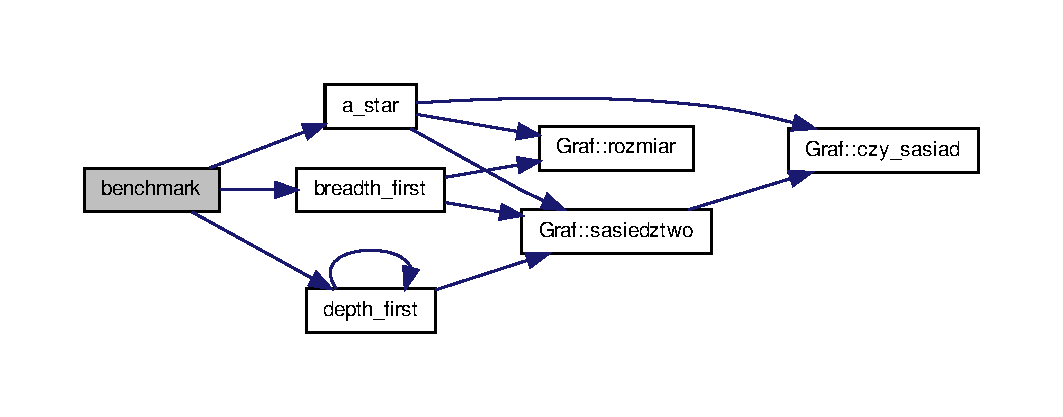
\includegraphics[width=350pt]{benchmark_8cpp_a4a33bba40119da5e2debd21d9ab45cdb_cgraph}
\end{center}
\end{figure}




\-Oto graf wywoływań tej funkcji\-:\nopagebreak
\begin{figure}[H]
\begin{center}
\leavevmode
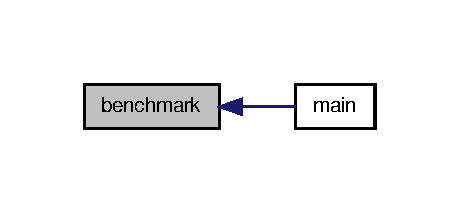
\includegraphics[width=220pt]{benchmark_8cpp_a4a33bba40119da5e2debd21d9ab45cdb_icgraph}
\end{center}
\end{figure}



\hypertarget{benchmark_8h}{\section{\-Dokumentacja pliku benchmark.\-h}
\label{benchmark_8h}\index{benchmark.\-h@{benchmark.\-h}}
}


\-Plik naglowkowy \-Benchmark.  


{\ttfamily \#include \char`\"{}graf.\-h\char`\"{}}\*
{\ttfamily \#include $<$iostream$>$}\*
\-Wykres zależności załączania dla benchmark.\-h\-:\nopagebreak
\begin{figure}[H]
\begin{center}
\leavevmode
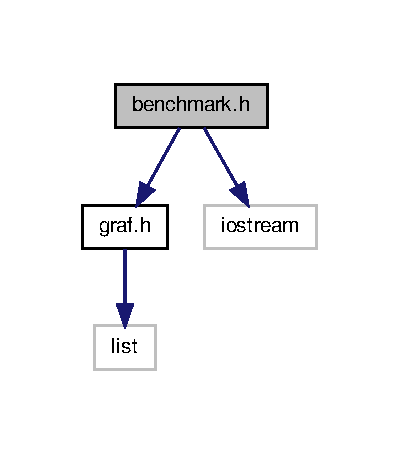
\includegraphics[width=192pt]{benchmark_8h__incl}
\end{center}
\end{figure}
\-Ten wykres pokazuje, które pliki bezpośrednio lub pośrednio załączają ten plik\-:\nopagebreak
\begin{figure}[H]
\begin{center}
\leavevmode
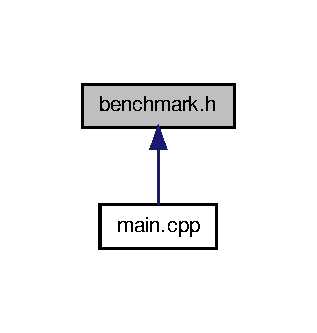
\includegraphics[width=152pt]{benchmark_8h__dep__incl}
\end{center}
\end{figure}
\subsection*{\-Funkcje}
\begin{DoxyCompactItemize}
\item 
void \hyperlink{benchmark_8h_a4a33bba40119da5e2debd21d9ab45cdb}{benchmark} (\hyperlink{class_graf}{\-Graf} \&cos, int poczatek, int koniec, std\-::ostream \&out)
\end{DoxyCompactItemize}


\subsection{\-Opis szczegółowy}


\-Definicja w pliku \hyperlink{benchmark_8h_source}{benchmark.\-h}.



\subsection{\-Dokumentacja funkcji}
\hypertarget{benchmark_8h_a4a33bba40119da5e2debd21d9ab45cdb}{\index{benchmark.\-h@{benchmark.\-h}!benchmark@{benchmark}}
\index{benchmark@{benchmark}!benchmark.h@{benchmark.\-h}}
\subsubsection[{benchmark}]{\setlength{\rightskip}{0pt plus 5cm}void {\bf benchmark} (
\begin{DoxyParamCaption}
\item[{{\bf \-Graf} \&}]{cos, }
\item[{int}]{poczatek, }
\item[{int}]{koniec, }
\item[{std\-::ostream \&}]{out}
\end{DoxyParamCaption}
)}}\label{benchmark_8h_a4a33bba40119da5e2debd21d9ab45cdb}


\-Definicja w linii 15 pliku benchmark.\-cpp.



\-Oto graf wywołań dla tej funkcji\-:\nopagebreak
\begin{figure}[H]
\begin{center}
\leavevmode
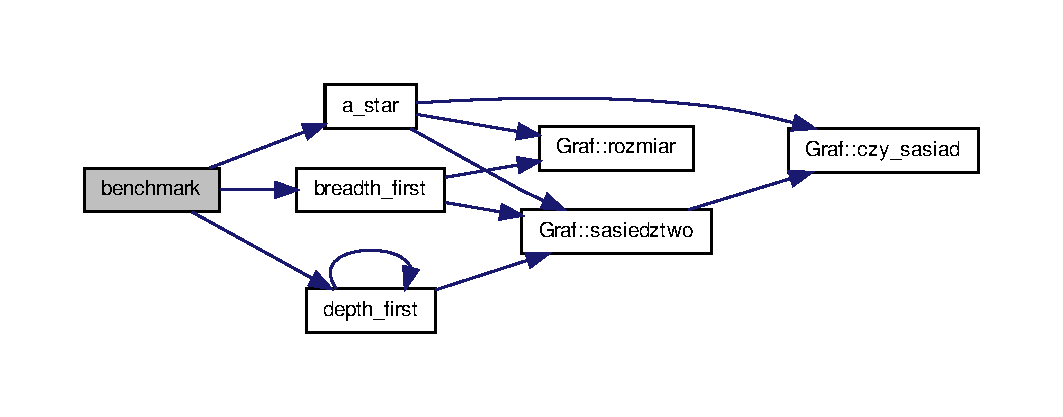
\includegraphics[width=350pt]{benchmark_8h_a4a33bba40119da5e2debd21d9ab45cdb_cgraph}
\end{center}
\end{figure}




\-Oto graf wywoływań tej funkcji\-:\nopagebreak
\begin{figure}[H]
\begin{center}
\leavevmode
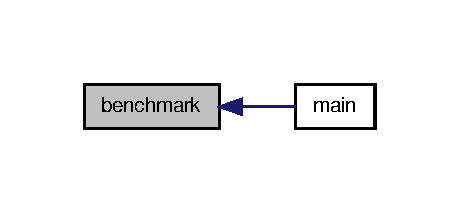
\includegraphics[width=220pt]{benchmark_8h_a4a33bba40119da5e2debd21d9ab45cdb_icgraph}
\end{center}
\end{figure}



\hypertarget{graf_8cpp}{\section{\-Dokumentacja pliku graf.\-cpp}
\label{graf_8cpp}\index{graf.\-cpp@{graf.\-cpp}}
}


\-Definicje poszczegolnych funkcji dla klasy \hyperlink{class_graf}{\-Graf}.  


{\ttfamily \#include $<$list$>$}\*
{\ttfamily \#include \char`\"{}graf.\-h\char`\"{}}\*
\-Wykres zależności załączania dla graf.\-cpp\-:\nopagebreak
\begin{figure}[H]
\begin{center}
\leavevmode
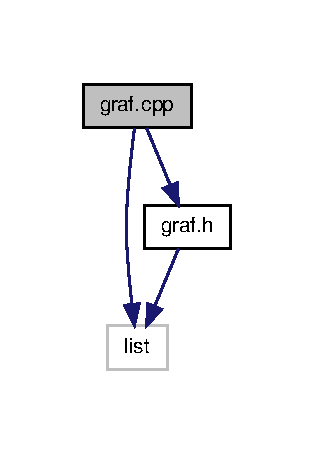
\includegraphics[width=150pt]{graf_8cpp__incl}
\end{center}
\end{figure}


\subsection{\-Opis szczegółowy}


\-Definicja w pliku \hyperlink{graf_8cpp_source}{graf.\-cpp}.


\hypertarget{graf_8h}{\section{\-Dokumentacja pliku graf.\-h}
\label{graf_8h}\index{graf.\-h@{graf.\-h}}
}


\-Plik naglowkowy klasy \-Graf.\-Klasa \hyperlink{class_graf}{\-Graf} zawierajaca definicje poszczegolnych funkcji.  


{\ttfamily \#include $<$list$>$}\*
\-Wykres zależności załączania dla graf.\-h\-:\nopagebreak
\begin{figure}[H]
\begin{center}
\leavevmode
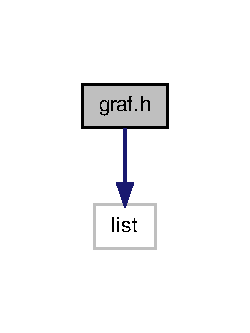
\includegraphics[width=120pt]{graf_8h__incl}
\end{center}
\end{figure}
\-Ten wykres pokazuje, które pliki bezpośrednio lub pośrednio załączają ten plik\-:\nopagebreak
\begin{figure}[H]
\begin{center}
\leavevmode
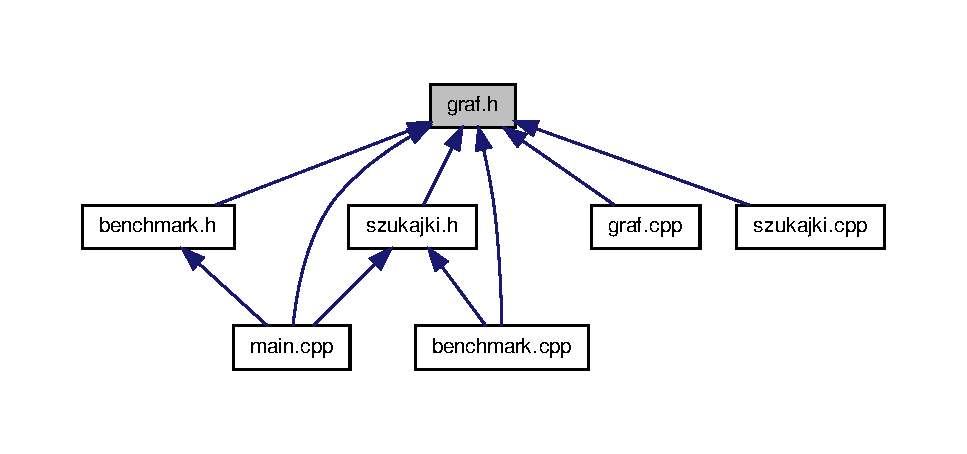
\includegraphics[width=350pt]{graf_8h__dep__incl}
\end{center}
\end{figure}
\subsection*{\-Komponenty}
\begin{DoxyCompactItemize}
\item 
class \hyperlink{class_graf}{\-Graf}
\begin{DoxyCompactList}\small\item\em \-Deklaracja klasy \hyperlink{class_graf}{\-Graf}. \end{DoxyCompactList}\end{DoxyCompactItemize}


\subsection{\-Opis szczegółowy}


\-Definicja w pliku \hyperlink{graf_8h_source}{graf.\-h}.


\hypertarget{main_8cpp}{\section{\-Dokumentacja pliku /home/martyna/\-Pulpit/calka/prj/main.cpp}
\label{main_8cpp}\index{/home/martyna/\-Pulpit/calka/prj/main.\-cpp@{/home/martyna/\-Pulpit/calka/prj/main.\-cpp}}
}


\-Plik zawiera glowna funkcje programu.  


{\ttfamily \#include $<$iostream$>$}\*
{\ttfamily \#include \char`\"{}integral.\-h\char`\"{}}\*
\-Wykres zależności załączania dla main.\-cpp\-:\nopagebreak
\begin{figure}[H]
\begin{center}
\leavevmode
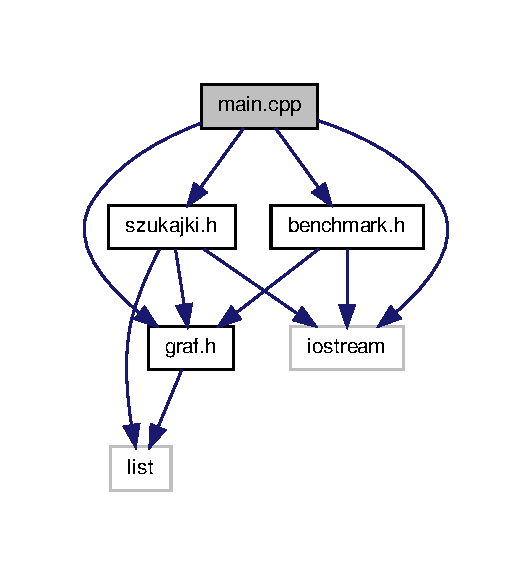
\includegraphics[width=272pt]{main_8cpp__incl}
\end{center}
\end{figure}
\subsection*{\-Funkcje}
\begin{DoxyCompactItemize}
\item 
double \hyperlink{main_8cpp_a80abd7257657e8a5b78f917731d87ba5}{\-F} (double x)
\item 
int \hyperlink{main_8cpp_ae66f6b31b5ad750f1fe042a706a4e3d4}{main} ()
\end{DoxyCompactItemize}


\subsection{\-Opis szczegółowy}
\-Plik zawiera glowna funkcje programu. 

\-Definicja w pliku \hyperlink{main_8cpp_source}{main.\-cpp}.



\subsection{\-Dokumentacja funkcji}
\hypertarget{main_8cpp_a80abd7257657e8a5b78f917731d87ba5}{\index{main.\-cpp@{main.\-cpp}!\-F@{\-F}}
\index{\-F@{\-F}!main.cpp@{main.\-cpp}}
\subsubsection[{\-F}]{\setlength{\rightskip}{0pt plus 5cm}double {\bf \-F} (
\begin{DoxyParamCaption}
\item[{double}]{x}
\end{DoxyParamCaption}
)}}\label{main_8cpp_a80abd7257657e8a5b78f917731d87ba5}


\-Definicja w linii 11 pliku main.\-cpp.



\-Oto graf wywoływań tej funkcji\-:\nopagebreak
\begin{figure}[H]
\begin{center}
\leavevmode
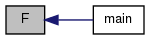
\includegraphics[width=184pt]{main_8cpp_a80abd7257657e8a5b78f917731d87ba5_icgraph}
\end{center}
\end{figure}


\hypertarget{main_8cpp_ae66f6b31b5ad750f1fe042a706a4e3d4}{\index{main.\-cpp@{main.\-cpp}!main@{main}}
\index{main@{main}!main.cpp@{main.\-cpp}}
\subsubsection[{main}]{\setlength{\rightskip}{0pt plus 5cm}int {\bf main} (
\begin{DoxyParamCaption}
{}
\end{DoxyParamCaption}
)}}\label{main_8cpp_ae66f6b31b5ad750f1fe042a706a4e3d4}


\-Definicja w linii 15 pliku main.\-cpp.



\-Oto graf wywołań dla tej funkcji\-:\nopagebreak
\begin{figure}[H]
\begin{center}
\leavevmode
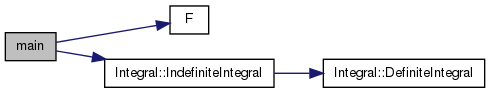
\includegraphics[width=350pt]{main_8cpp_ae66f6b31b5ad750f1fe042a706a4e3d4_cgraph}
\end{center}
\end{figure}



\hypertarget{szukajki_8cpp}{\section{\-Dokumentacja pliku szukajki.\-cpp}
\label{szukajki_8cpp}\index{szukajki.\-cpp@{szukajki.\-cpp}}
}


\-Szukajki \-Zawiera najważniejsze fukcje programu. \-Trzy przeszukiwania grafu -\/ depth first, breadth first, \-A$\ast$.  


{\ttfamily \#include \char`\"{}graf.\-h\char`\"{}}\*
{\ttfamily \#include $<$iostream$>$}\*
{\ttfamily \#include $<$list$>$}\*
{\ttfamily \#include $<$algorithm$>$}\*
{\ttfamily \#include $<$limits$>$}\*
{\ttfamily \#include $<$set$>$}\*
\-Wykres zależności załączania dla szukajki.\-cpp\-:\nopagebreak
\begin{figure}[H]
\begin{center}
\leavevmode
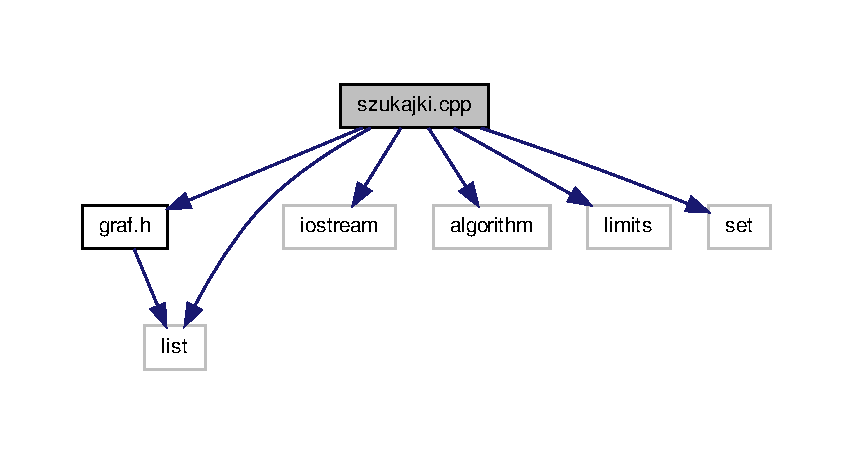
\includegraphics[width=350pt]{szukajki_8cpp__incl}
\end{center}
\end{figure}
\subsection*{\-Definicje}
\begin{DoxyCompactItemize}
\item 
\#define \hyperlink{szukajki_8cpp_a666d9e148914053f86c5343a0aed4838}{\-W\-A\-L\-L\-Y}~15
\end{DoxyCompactItemize}
\subsection*{\-Funkcje}
\begin{DoxyCompactItemize}
\item 
std\-::list$<$ int $>$ \hyperlink{szukajki_8cpp_a536e69aa7f75ebf65321838eaa5b535b}{depth\-\_\-first} (\hyperlink{class_graf}{\-Graf} \&cos, int poczatek, int koniec, std\-::list$<$ int $>$ historia)
\item 
std\-::list$<$ int $>$ \hyperlink{szukajki_8cpp_a7b032574cc2090ceeb7725d81705e791}{depth\-\_\-first} (\hyperlink{class_graf}{\-Graf} \&cos, int poczatek, int koniec)
\item 
std\-::list$<$ int $>$ \hyperlink{szukajki_8cpp_a520d7f85b9377df6341c9935d2a8a7f6}{breadth\-\_\-first} (\hyperlink{class_graf}{\-Graf} \&cos, const int poczatek, const int koniec)
\item 
double \hyperlink{szukajki_8cpp_a020c61195a8975d1449ea395a81aba30}{licz\-Koszt} (\hyperlink{class_graf}{\-Graf} \&cos, std\-::list$<$ int $>$ droga)
\item 
std\-::list$<$ int $>$ \hyperlink{szukajki_8cpp_a5b32516af3ae3ac383db8cd7a6827bec}{a\-\_\-star} (\hyperlink{class_graf}{\-Graf} \&cos, int poczatek, int koniec)
\end{DoxyCompactItemize}


\subsection{\-Opis szczegółowy}


\-Definicja w pliku \hyperlink{szukajki_8cpp_source}{szukajki.\-cpp}.



\subsection{\-Dokumentacja definicji}
\hypertarget{szukajki_8cpp_a666d9e148914053f86c5343a0aed4838}{\index{szukajki.\-cpp@{szukajki.\-cpp}!\-W\-A\-L\-L\-Y@{\-W\-A\-L\-L\-Y}}
\index{\-W\-A\-L\-L\-Y@{\-W\-A\-L\-L\-Y}!szukajki.cpp@{szukajki.\-cpp}}
\subsubsection[{\-W\-A\-L\-L\-Y}]{\setlength{\rightskip}{0pt plus 5cm}\#define {\bf \-W\-A\-L\-L\-Y}~15}}\label{szukajki_8cpp_a666d9e148914053f86c5343a0aed4838}


\-Definicja w linii 16 pliku szukajki.\-cpp.



\subsection{\-Dokumentacja funkcji}
\hypertarget{szukajki_8cpp_a5b32516af3ae3ac383db8cd7a6827bec}{\index{szukajki.\-cpp@{szukajki.\-cpp}!a\-\_\-star@{a\-\_\-star}}
\index{a\-\_\-star@{a\-\_\-star}!szukajki.cpp@{szukajki.\-cpp}}
\subsubsection[{a\-\_\-star}]{\setlength{\rightskip}{0pt plus 5cm}std\-::list$<$int$>$ {\bf a\-\_\-star} (
\begin{DoxyParamCaption}
\item[{{\bf \-Graf} \&}]{cos, }
\item[{int}]{poczatek, }
\item[{int}]{koniec}
\end{DoxyParamCaption}
)}}\label{szukajki_8cpp_a5b32516af3ae3ac383db8cd7a6827bec}


\-Definicja w linii 103 pliku szukajki.\-cpp.



\-Oto graf wywołań dla tej funkcji\-:\nopagebreak
\begin{figure}[H]
\begin{center}
\leavevmode
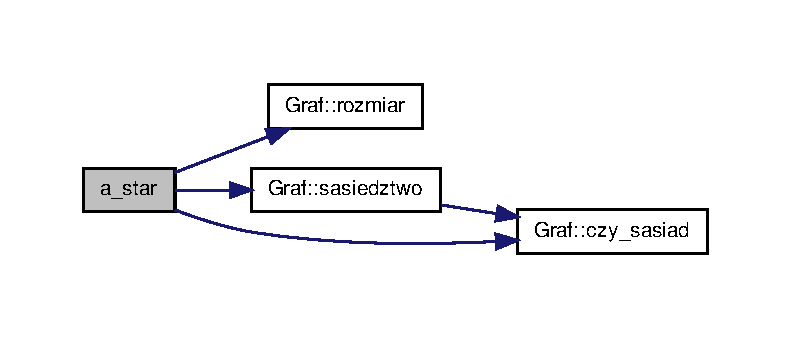
\includegraphics[width=350pt]{szukajki_8cpp_a5b32516af3ae3ac383db8cd7a6827bec_cgraph}
\end{center}
\end{figure}




\-Oto graf wywoływań tej funkcji\-:\nopagebreak
\begin{figure}[H]
\begin{center}
\leavevmode
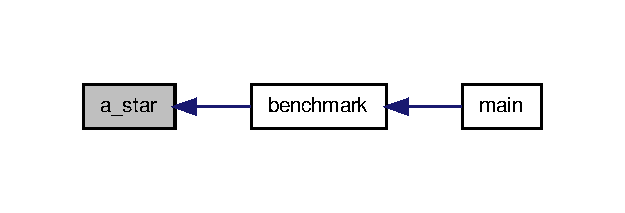
\includegraphics[width=300pt]{szukajki_8cpp_a5b32516af3ae3ac383db8cd7a6827bec_icgraph}
\end{center}
\end{figure}


\hypertarget{szukajki_8cpp_a520d7f85b9377df6341c9935d2a8a7f6}{\index{szukajki.\-cpp@{szukajki.\-cpp}!breadth\-\_\-first@{breadth\-\_\-first}}
\index{breadth\-\_\-first@{breadth\-\_\-first}!szukajki.cpp@{szukajki.\-cpp}}
\subsubsection[{breadth\-\_\-first}]{\setlength{\rightskip}{0pt plus 5cm}std\-::list$<$int$>$ {\bf breadth\-\_\-first} (
\begin{DoxyParamCaption}
\item[{{\bf \-Graf} \&}]{cos, }
\item[{const int}]{poczatek, }
\item[{const int}]{koniec}
\end{DoxyParamCaption}
)}}\label{szukajki_8cpp_a520d7f85b9377df6341c9935d2a8a7f6}


\-Definicja w linii 32 pliku szukajki.\-cpp.



\-Oto graf wywołań dla tej funkcji\-:\nopagebreak
\begin{figure}[H]
\begin{center}
\leavevmode
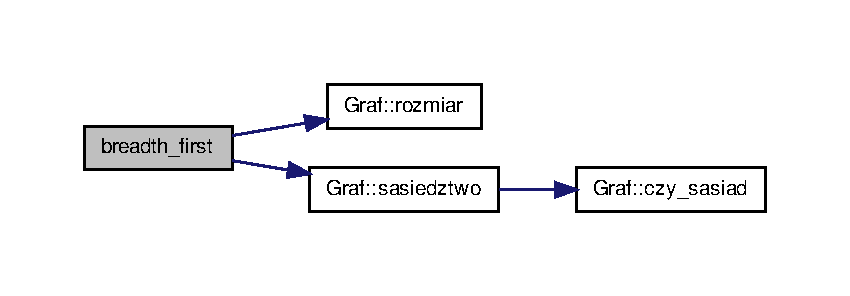
\includegraphics[width=350pt]{szukajki_8cpp_a520d7f85b9377df6341c9935d2a8a7f6_cgraph}
\end{center}
\end{figure}




\-Oto graf wywoływań tej funkcji\-:\nopagebreak
\begin{figure}[H]
\begin{center}
\leavevmode
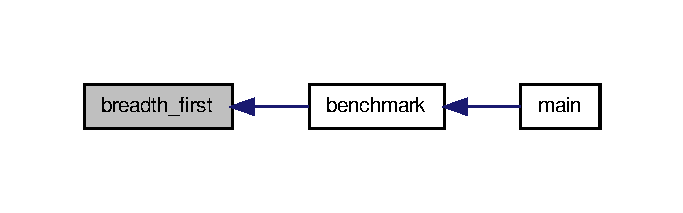
\includegraphics[width=328pt]{szukajki_8cpp_a520d7f85b9377df6341c9935d2a8a7f6_icgraph}
\end{center}
\end{figure}


\hypertarget{szukajki_8cpp_a536e69aa7f75ebf65321838eaa5b535b}{\index{szukajki.\-cpp@{szukajki.\-cpp}!depth\-\_\-first@{depth\-\_\-first}}
\index{depth\-\_\-first@{depth\-\_\-first}!szukajki.cpp@{szukajki.\-cpp}}
\subsubsection[{depth\-\_\-first}]{\setlength{\rightskip}{0pt plus 5cm}std\-::list$<$int$>$ {\bf depth\-\_\-first} (
\begin{DoxyParamCaption}
\item[{{\bf \-Graf} \&}]{cos, }
\item[{int}]{poczatek, }
\item[{int}]{koniec, }
\item[{std\-::list$<$ int $>$}]{historia}
\end{DoxyParamCaption}
)}}\label{szukajki_8cpp_a536e69aa7f75ebf65321838eaa5b535b}


\-Definicja w linii 17 pliku szukajki.\-cpp.



\-Oto graf wywołań dla tej funkcji\-:\nopagebreak
\begin{figure}[H]
\begin{center}
\leavevmode
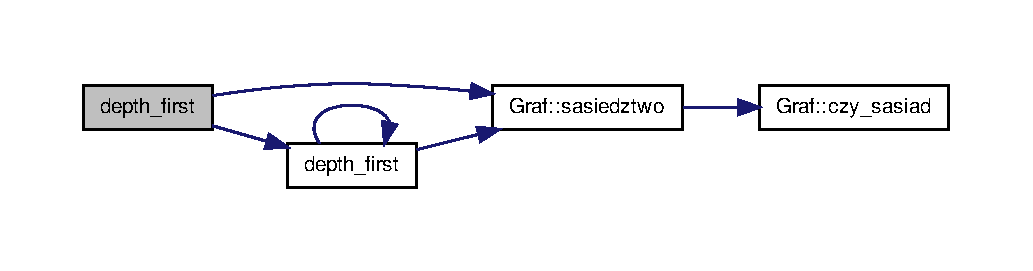
\includegraphics[width=350pt]{szukajki_8cpp_a536e69aa7f75ebf65321838eaa5b535b_cgraph}
\end{center}
\end{figure}




\-Oto graf wywoływań tej funkcji\-:\nopagebreak
\begin{figure}[H]
\begin{center}
\leavevmode
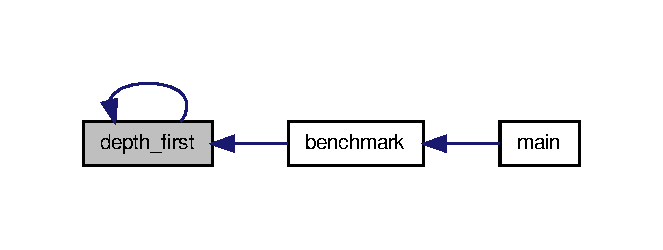
\includegraphics[width=318pt]{szukajki_8cpp_a536e69aa7f75ebf65321838eaa5b535b_icgraph}
\end{center}
\end{figure}


\hypertarget{szukajki_8cpp_a7b032574cc2090ceeb7725d81705e791}{\index{szukajki.\-cpp@{szukajki.\-cpp}!depth\-\_\-first@{depth\-\_\-first}}
\index{depth\-\_\-first@{depth\-\_\-first}!szukajki.cpp@{szukajki.\-cpp}}
\subsubsection[{depth\-\_\-first}]{\setlength{\rightskip}{0pt plus 5cm}std\-::list$<$int$>$ {\bf depth\-\_\-first} (
\begin{DoxyParamCaption}
\item[{{\bf \-Graf} \&}]{cos, }
\item[{int}]{poczatek, }
\item[{int}]{koniec}
\end{DoxyParamCaption}
)}}\label{szukajki_8cpp_a7b032574cc2090ceeb7725d81705e791}


\-Definicja w linii 28 pliku szukajki.\-cpp.



\-Oto graf wywołań dla tej funkcji\-:\nopagebreak
\begin{figure}[H]
\begin{center}
\leavevmode
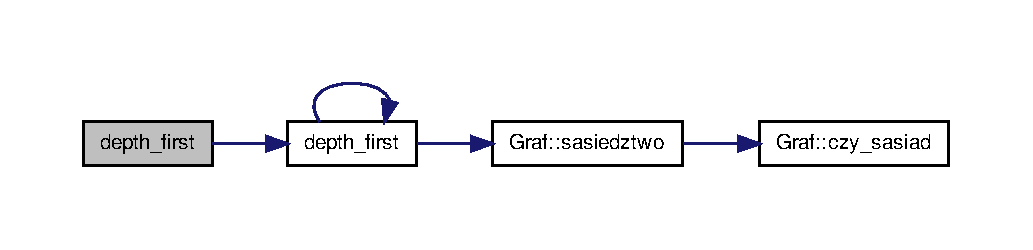
\includegraphics[width=350pt]{szukajki_8cpp_a7b032574cc2090ceeb7725d81705e791_cgraph}
\end{center}
\end{figure}


\hypertarget{szukajki_8cpp_a020c61195a8975d1449ea395a81aba30}{\index{szukajki.\-cpp@{szukajki.\-cpp}!licz\-Koszt@{licz\-Koszt}}
\index{licz\-Koszt@{licz\-Koszt}!szukajki.cpp@{szukajki.\-cpp}}
\subsubsection[{licz\-Koszt}]{\setlength{\rightskip}{0pt plus 5cm}double {\bf licz\-Koszt} (
\begin{DoxyParamCaption}
\item[{{\bf \-Graf} \&}]{cos, }
\item[{std\-::list$<$ int $>$}]{droga}
\end{DoxyParamCaption}
)}}\label{szukajki_8cpp_a020c61195a8975d1449ea395a81aba30}


\-Definicja w linii 63 pliku szukajki.\-cpp.



\-Oto graf wywołań dla tej funkcji\-:\nopagebreak
\begin{figure}[H]
\begin{center}
\leavevmode
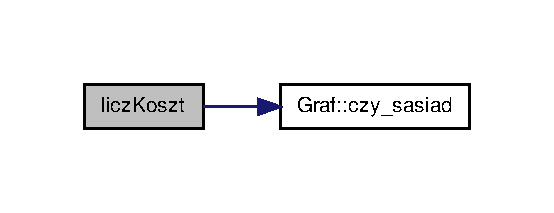
\includegraphics[width=266pt]{szukajki_8cpp_a020c61195a8975d1449ea395a81aba30_cgraph}
\end{center}
\end{figure}



\hypertarget{szukajki_8h}{\section{\-Dokumentacja pliku szukajki.\-h}
\label{szukajki_8h}\index{szukajki.\-h@{szukajki.\-h}}
}


\-Plik zawiera definicje funkcji szukajki.  


{\ttfamily \#include \char`\"{}graf.\-h\char`\"{}}\*
{\ttfamily \#include $<$iostream$>$}\*
{\ttfamily \#include $<$list$>$}\*
\-Wykres zależności załączania dla szukajki.\-h\-:\nopagebreak
\begin{figure}[H]
\begin{center}
\leavevmode
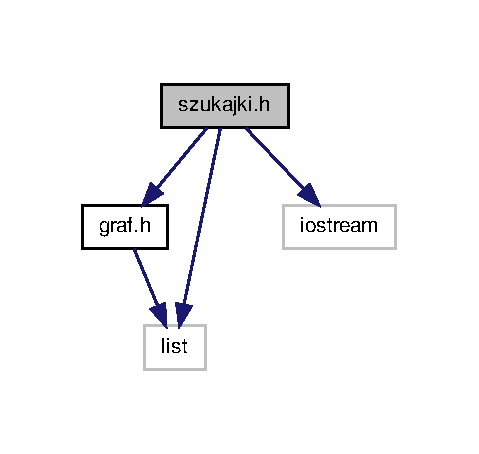
\includegraphics[width=230pt]{szukajki_8h__incl}
\end{center}
\end{figure}
\-Ten wykres pokazuje, które pliki bezpośrednio lub pośrednio załączają ten plik\-:\nopagebreak
\begin{figure}[H]
\begin{center}
\leavevmode
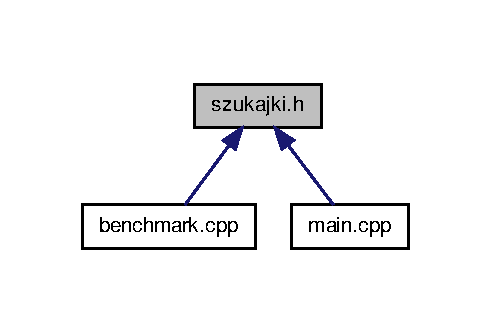
\includegraphics[width=236pt]{szukajki_8h__dep__incl}
\end{center}
\end{figure}
\subsection*{\-Funkcje}
\begin{DoxyCompactItemize}
\item 
std\-::list$<$ int $>$ \hyperlink{szukajki_8h_a536e69aa7f75ebf65321838eaa5b535b}{depth\-\_\-first} (\hyperlink{class_graf}{\-Graf} \&cos, int poczatek, int koniec, std\-::list$<$ int $>$ historia)
\item 
std\-::list$<$ int $>$ \hyperlink{szukajki_8h_a7b032574cc2090ceeb7725d81705e791}{depth\-\_\-first} (\hyperlink{class_graf}{\-Graf} \&cos, int poczatek, int koniec)
\item 
std\-::list$<$ int $>$ \hyperlink{szukajki_8h_a520d7f85b9377df6341c9935d2a8a7f6}{breadth\-\_\-first} (\hyperlink{class_graf}{\-Graf} \&cos, const int poczatek, const int koniec)
\item 
double \hyperlink{szukajki_8h_a020c61195a8975d1449ea395a81aba30}{licz\-Koszt} (\hyperlink{class_graf}{\-Graf} \&cos, std\-::list$<$ int $>$ droga)
\item 
std\-::list$<$ int $>$ \hyperlink{szukajki_8h_a5b32516af3ae3ac383db8cd7a6827bec}{a\-\_\-star} (\hyperlink{class_graf}{\-Graf} \&cos, int poczatek, int koniec)
\end{DoxyCompactItemize}


\subsection{\-Opis szczegółowy}


\-Definicja w pliku \hyperlink{szukajki_8h_source}{szukajki.\-h}.



\subsection{\-Dokumentacja funkcji}
\hypertarget{szukajki_8h_a5b32516af3ae3ac383db8cd7a6827bec}{\index{szukajki.\-h@{szukajki.\-h}!a\-\_\-star@{a\-\_\-star}}
\index{a\-\_\-star@{a\-\_\-star}!szukajki.h@{szukajki.\-h}}
\subsubsection[{a\-\_\-star}]{\setlength{\rightskip}{0pt plus 5cm}std\-::list$<$int$>$ {\bf a\-\_\-star} (
\begin{DoxyParamCaption}
\item[{{\bf \-Graf} \&}]{cos, }
\item[{int}]{poczatek, }
\item[{int}]{koniec}
\end{DoxyParamCaption}
)}}\label{szukajki_8h_a5b32516af3ae3ac383db8cd7a6827bec}


\-Definicja w linii 103 pliku szukajki.\-cpp.



\-Oto graf wywołań dla tej funkcji\-:\nopagebreak
\begin{figure}[H]
\begin{center}
\leavevmode
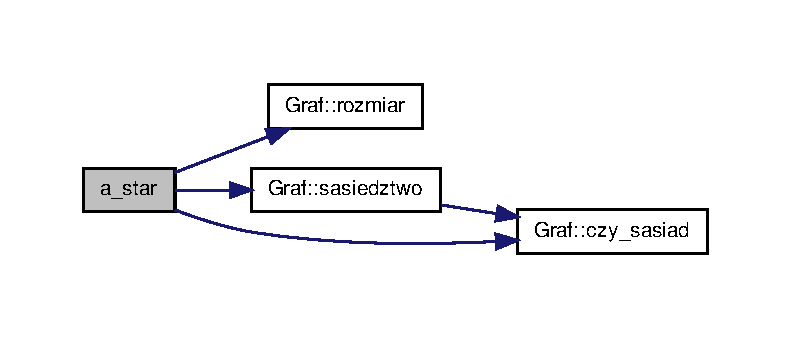
\includegraphics[width=350pt]{szukajki_8h_a5b32516af3ae3ac383db8cd7a6827bec_cgraph}
\end{center}
\end{figure}




\-Oto graf wywoływań tej funkcji\-:\nopagebreak
\begin{figure}[H]
\begin{center}
\leavevmode
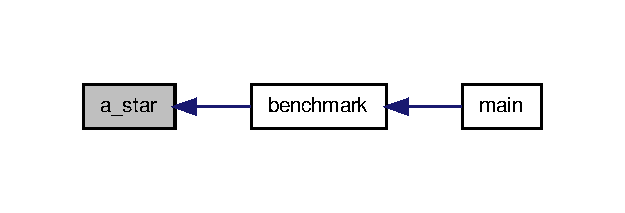
\includegraphics[width=300pt]{szukajki_8h_a5b32516af3ae3ac383db8cd7a6827bec_icgraph}
\end{center}
\end{figure}


\hypertarget{szukajki_8h_a520d7f85b9377df6341c9935d2a8a7f6}{\index{szukajki.\-h@{szukajki.\-h}!breadth\-\_\-first@{breadth\-\_\-first}}
\index{breadth\-\_\-first@{breadth\-\_\-first}!szukajki.h@{szukajki.\-h}}
\subsubsection[{breadth\-\_\-first}]{\setlength{\rightskip}{0pt plus 5cm}std\-::list$<$int$>$ {\bf breadth\-\_\-first} (
\begin{DoxyParamCaption}
\item[{{\bf \-Graf} \&}]{cos, }
\item[{const int}]{poczatek, }
\item[{const int}]{koniec}
\end{DoxyParamCaption}
)}}\label{szukajki_8h_a520d7f85b9377df6341c9935d2a8a7f6}


\-Definicja w linii 32 pliku szukajki.\-cpp.



\-Oto graf wywołań dla tej funkcji\-:\nopagebreak
\begin{figure}[H]
\begin{center}
\leavevmode
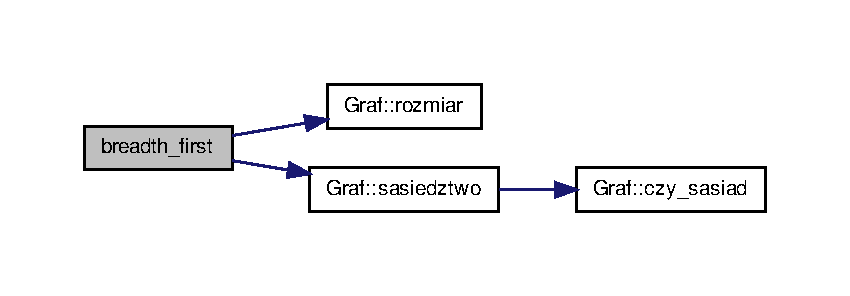
\includegraphics[width=350pt]{szukajki_8h_a520d7f85b9377df6341c9935d2a8a7f6_cgraph}
\end{center}
\end{figure}




\-Oto graf wywoływań tej funkcji\-:\nopagebreak
\begin{figure}[H]
\begin{center}
\leavevmode
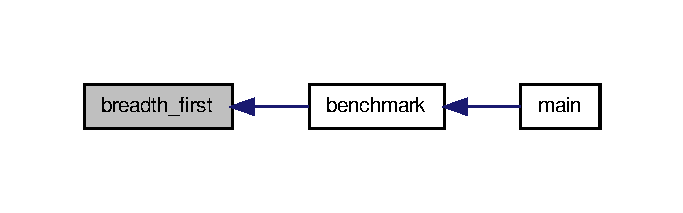
\includegraphics[width=328pt]{szukajki_8h_a520d7f85b9377df6341c9935d2a8a7f6_icgraph}
\end{center}
\end{figure}


\hypertarget{szukajki_8h_a536e69aa7f75ebf65321838eaa5b535b}{\index{szukajki.\-h@{szukajki.\-h}!depth\-\_\-first@{depth\-\_\-first}}
\index{depth\-\_\-first@{depth\-\_\-first}!szukajki.h@{szukajki.\-h}}
\subsubsection[{depth\-\_\-first}]{\setlength{\rightskip}{0pt plus 5cm}std\-::list$<$int$>$ {\bf depth\-\_\-first} (
\begin{DoxyParamCaption}
\item[{{\bf \-Graf} \&}]{cos, }
\item[{int}]{poczatek, }
\item[{int}]{koniec, }
\item[{std\-::list$<$ int $>$}]{historia}
\end{DoxyParamCaption}
)}}\label{szukajki_8h_a536e69aa7f75ebf65321838eaa5b535b}


\-Definicja w linii 17 pliku szukajki.\-cpp.



\-Oto graf wywołań dla tej funkcji\-:\nopagebreak
\begin{figure}[H]
\begin{center}
\leavevmode
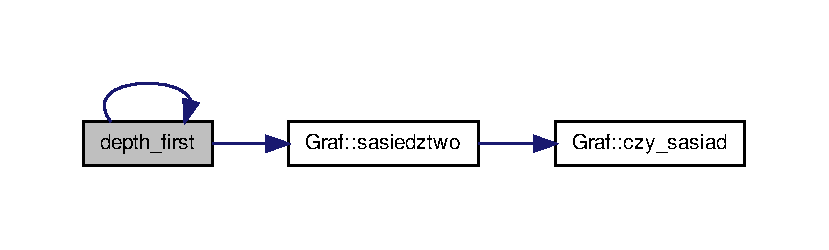
\includegraphics[width=350pt]{szukajki_8h_a536e69aa7f75ebf65321838eaa5b535b_cgraph}
\end{center}
\end{figure}




\-Oto graf wywoływań tej funkcji\-:\nopagebreak
\begin{figure}[H]
\begin{center}
\leavevmode
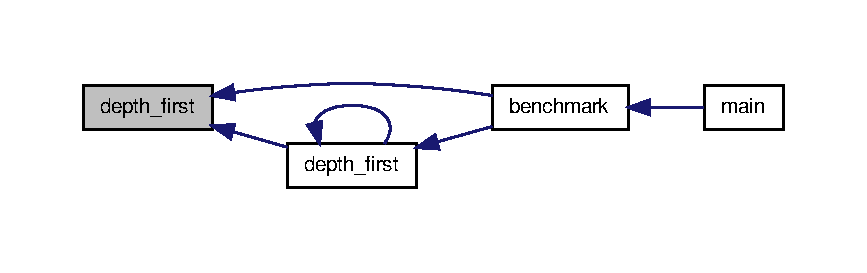
\includegraphics[width=350pt]{szukajki_8h_a536e69aa7f75ebf65321838eaa5b535b_icgraph}
\end{center}
\end{figure}


\hypertarget{szukajki_8h_a7b032574cc2090ceeb7725d81705e791}{\index{szukajki.\-h@{szukajki.\-h}!depth\-\_\-first@{depth\-\_\-first}}
\index{depth\-\_\-first@{depth\-\_\-first}!szukajki.h@{szukajki.\-h}}
\subsubsection[{depth\-\_\-first}]{\setlength{\rightskip}{0pt plus 5cm}std\-::list$<$int$>$ {\bf depth\-\_\-first} (
\begin{DoxyParamCaption}
\item[{{\bf \-Graf} \&}]{cos, }
\item[{int}]{poczatek, }
\item[{int}]{koniec}
\end{DoxyParamCaption}
)}}\label{szukajki_8h_a7b032574cc2090ceeb7725d81705e791}


\-Definicja w linii 28 pliku szukajki.\-cpp.



\-Oto graf wywołań dla tej funkcji\-:\nopagebreak
\begin{figure}[H]
\begin{center}
\leavevmode
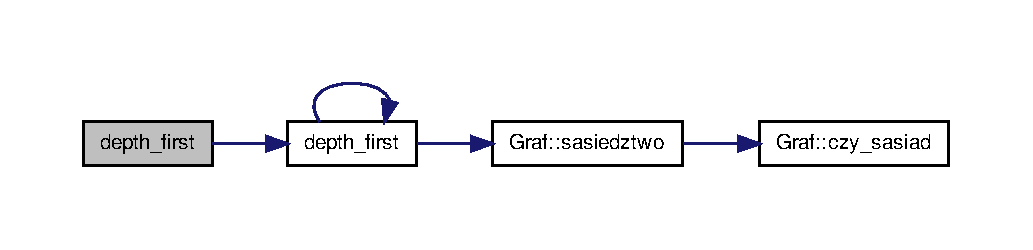
\includegraphics[width=350pt]{szukajki_8h_a7b032574cc2090ceeb7725d81705e791_cgraph}
\end{center}
\end{figure}


\hypertarget{szukajki_8h_a020c61195a8975d1449ea395a81aba30}{\index{szukajki.\-h@{szukajki.\-h}!licz\-Koszt@{licz\-Koszt}}
\index{licz\-Koszt@{licz\-Koszt}!szukajki.h@{szukajki.\-h}}
\subsubsection[{licz\-Koszt}]{\setlength{\rightskip}{0pt plus 5cm}double {\bf licz\-Koszt} (
\begin{DoxyParamCaption}
\item[{{\bf \-Graf} \&}]{cos, }
\item[{std\-::list$<$ int $>$}]{droga}
\end{DoxyParamCaption}
)}}\label{szukajki_8h_a020c61195a8975d1449ea395a81aba30}


\-Definicja w linii 63 pliku szukajki.\-cpp.



\-Oto graf wywołań dla tej funkcji\-:\nopagebreak
\begin{figure}[H]
\begin{center}
\leavevmode
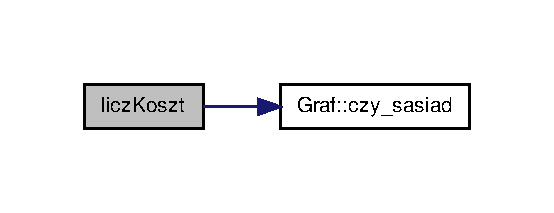
\includegraphics[width=266pt]{szukajki_8h_a020c61195a8975d1449ea395a81aba30_cgraph}
\end{center}
\end{figure}



\printindex
\end{document}
